\section{Introduction}
\subsection{Environnement du stage}

Ce travail est la synthèse de mon stage de première année de Master, durant lequel j’ai intégré l’équipe de la professeure Thérèse Commes du laboratoire Bio2M,  
rattaché à l’Institut national de la santé et de la recherche médicale (INSERM). J’ai eu la chance d’être accompagné dans mon apprentissage par Anthony Boureux, enseignant-chercheur.  
L’équipe collabore  avec des services cliniques et des plateformes hospitalières, ce qui favorise la résolution de problématiques liées au diagnostic médical.  
Ainsi, j’ai eu l’occasion de contribuer à un projet de recherche translationnelle que Bio2M mène en partenariat avec le CHU de Nîmes. Ce travail est en lien direct avec des enjeux diagnostiques,
 puisqu’il concerne une maladie neurodégénérative : la sclérose latérale amyotrophique (SLA).  
Les différentes missions qui m’ont été confiées s’inscrivent dans le champ de la transcriptomique, et plus particulièrement dans le cadre de l’analyse d’expression génique appliquée à la SLA,  
l’idée étant d’initier une stratégie permettant de détecter une expression différentielle à l’échelle de certains gènes d’intérêt dans la SLA, avec des contraintes à la fois techniques et biologiques,  
pour \textit{in fine} tenter d’identifier la causalité génétique chez les patients.

\subsection{Contexte biologique}

\begin{wrapfigure}{r}{0.50\textwidth} 
    \centering
    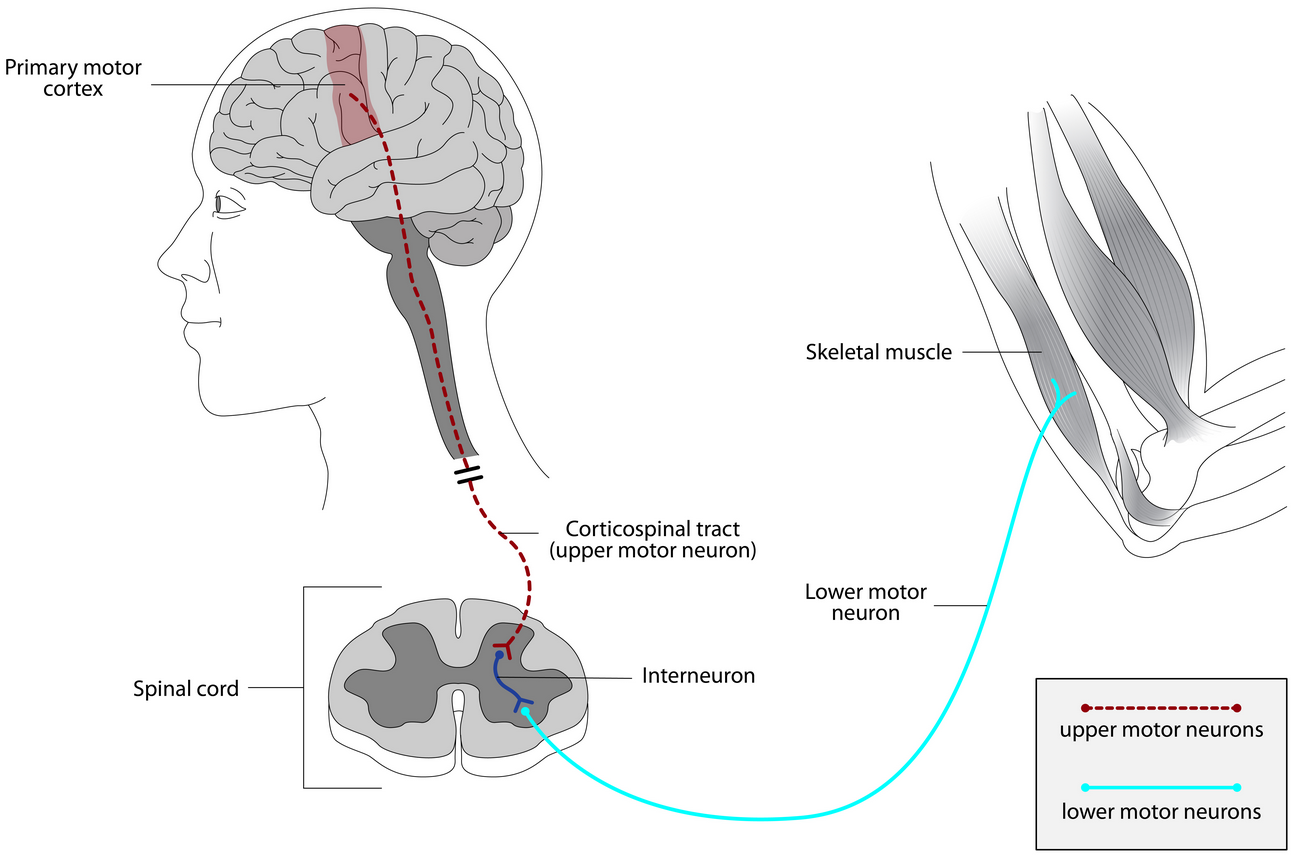
\includegraphics[width=1\linewidth]{Cortex_Spinal.jpg}
    \caption{\underline{Atteinte neuronale dans la SLA(P.Wicks, 2024)}}
    \label{fig:Cortex}
\end{wrapfigure}

Une maladie rare se définit par une \gls{prevalence} de 0,05~\% dans la population générale.  
Quatre-vingts pour cent de ces maladies sont d’origine génétique~\textsuperscript{\cite{SLA_protocole_2020}},  
et la SLA en fait partie : elle touche un individu sur 20\,000 en Europe~\textsuperscript{\cite{M.rare_prevalence_2023}},  
et sa prevalence mondiale varie de 1{,}57 à 11{,}8 pour 100\,000 selon les pays, de l’Iran aux États-Unis~\textsuperscript{\cite{SLA_prevalence_2023}}.  
C’est une maladie neurodégénérative causée par une atteinte du motoneurone central au niveau du cortex cérébral \textbf{(figure~\ref{fig:Cortex})},  
conduisant à une dégénérescence progressive des fonctions musculaires. Cette pathologie est très handicapante, tant sur le plan physique que social.  
En raison de sa gravité et des conséquences dévastatrices pour les patients et leur entourage, elle constitue un domaine de recherche de premier plan pour les généticiens cliniques.  
C’est pourquoi il est pertinent d’intégrer une approche transcriptomique afin d’augmenter le rendement diagnostique des formes génétiques de la maladie et de mieux en comprendre les mécanismes.
Notons que les gènes responsables de la SLA sont globalement bien documentés. À ce jour, une quarantaine de gènes ont été identifiés et associés à la maladie.  
Dans 90~\% des cas, leur implication est directe dans les formes familiales. Dans les 10~\% restants, on observe des formes dites sporadiques,  
où la causalité génétique est cette fois indirecte, via des perturbations de processus cellulaires clés tels que l’\gls{homeostasie} de l’ARN, le \gls{transport axonal} ou l’\gls{autophagie}.    
On observe également une forte hétérogénéité génétique dans cette maladie, perceptible à travers l’implication de gènes aux fonctions parfois très différentes,  
mais qui convergent toujours vers une dégénérescence neuronale. Les gènes les plus fréquemment impliqués sont \textit{SOD1}, \textit{TARDBP}, \textit{FUS} et \textit{C9ORF72}~\textsuperscript{\cite{SLA_protocole_2020}}.  
Majoritaires dans la maladie, ils constituent le socle des recherches génétiques pour tenter la mise au point de thérapies ciblées et faire progresser la compréhension ainsi que le diagnostic de cette pathologie.

\subsection{L’apport du RNA-Seq ciblé dans le périmètre de notre analyse}

D’un point de vue biologique, \textit{stricto sensu}, on sait que l’étape de transcription est fondatrice de la diversité protéomique ;  
elle constitue, de ce fait, une source majeure d’anomalies génétiques. À l’issue de ce mécanisme, un gène peut exprimer plusieurs isoformes, dont certaines peuvent avoir un impact pathologique.  
Tout l’objet de ce travail est de proposer une méthode pertinente pour détecter des différences d’expression de tel ou tel gènes, susceptibles d’aider le biologiste à établir un lien avec la maladie,  
notamment à travers une \gls{haploinsuffisance} ou, au contraire, une surexpression.\\
 
 \begin{wrapfigure}{l}{0.6\textwidth}
 
 \centering
 \vspace{-5mm}
 \scalebox{0.7}{ 
 \begin{tikzpicture}[node distance=1.5cm and 1cm]
     % Étapes principales
     \node (start) [startstop] {Prélèvement des échantillons : répétabilité biologique ?};
     \node (step1) [process, below of=start, text width=5cm, align=center] {Extraction de l'ARN total};
     \node (step2) [process, below of=step1, text width=5cm, align=center] {Enrichissement de l'ARNm};
     \node (step3) [process, below of=step2, text width=5cm, align=center] {Fragmentation de l'ARN};
     \node (step4) [process, below of=step3, text width=5cm, align=center] {Synthèse de l'ADNc};
     \node (step5) [process, below of=step4, text width=5cm, align=center] {Préparation de la librairie};
     \node (step6) [process, below of=step5, text width=5cm, align=center] {Quantification de la librairie};
     \node (step7) [process, below of=step6, text width=5cm, align=center] {Séquençage};
 
     % Biais techniques associés
     \node (note1) [techbias, right=1cm of step1, text width=5cm, align=center] {Pureté et concentration extraites};
     \node (note2) [techbias, right=1cm of step2, text width=5cm, align=center] {Perte d'ARNm non poly-A};
     \node (note3) [techbias, right=1cm of step3, text width=5cm, align=center] {Fragmentation imparfaite};
     \node (note4) [techbias, right=1cm of step4, text width=5cm, align=center] {Efficacité de la reverse transcription};
     \node (note5) [techbias, right=1cm of step5, text width=5cm, align=center] {Thermocycleur, variabilité inter-runs};
     \node (note6) [techbias, right=1cm of step6, text width=5cm, align=center] {Variabilité au dosage (Qubit, Bioanalyzer)};
     \node (note7) [techbias, right=1cm of step7, text width=5cm, align=center] {Erreurs liées au séquençage (Illumina, \textit{index hopping})};
     
     % Flèches principales
     \draw [arrow] (start) -- (step1);
     \draw [arrow] (step1) -- (step2);
     \draw [arrow] (step2) -- (step3);
     \draw [arrow] (step3) -- (step4);
     \draw [arrow] (step4) -- (step5);
     \draw [arrow] (step5) -- (step6);
     \draw [arrow] (step6) -- (step7);
 
     % Flèches vers les biais
     \draw [arrow] (step1) -- (note1);
     \draw [arrow] (step2) -- (note2);
     \draw [arrow] (step3) -- (note3);
     \draw [arrow] (step4) -- (note4);
     \draw [arrow] (step5) -- (note5);
     \draw [arrow] (step6) -- (note6);
     \draw [arrow] (step7) -- (note7);
 
     % Légende verticale à gauche
     \node[rectangle, rounded corners, draw=white, fill=gray!10,
           minimum width=10cm, minimum height=2cm,
           text width=2cm, align=center, anchor=north, rotate=90] 
           at ([xshift=-5.4cm, yshift=-6cm]) {\textbf{Processus technique}};
 
 \end{tikzpicture}
 }
 %\hspace{10cm}
 \caption{\underline{Processus expérimental du RNA-Seq et biais potentiels}}
 \label{fig:biaisRNA}
 \end{wrapfigure}

Supposons maintenant que l’on cherche à établir un profil d’expression génique pour notre quarantaine de gènes.  
Il convient alors de s’interroger sur le support de lecture de chacun de ces gènes, c’est-à-dire le nombre de fois qu’une région de l’ADN a été lue (ou comptée) au cours du séquençage.  
On s’attend logiquement à observer une distribution des lectures, interprétable comme le reflet du niveau d’expression de chaque gène étudié.  
En pratique, si l’on se fonde sur les données brutes, cette hypothèse s’avère souvent éloignée de la réalité : un certain nombre de variables~—~biologiques (rythme circadien, état physiologique, etc.) ou expérimentales (moment du prélèvement, conditions de manipulation, etc.)~—~influencent cette distribution théorique, introduisant une dispersion non négligeable dans le jeu de données.

Par ailleurs, le traitement bioinformatique peut lui aussi fausser le profil d’expression, notamment à travers les choix opérés lors de l’étape d’alignement~—~comme nous le verrons.  
La \textbf{figure~\ref{fig:biaisRNA}} illustre quelques-uns des biais, non exhaustifs, susceptibles d’affecter la quantification de l’expression génique.  
On comprend à travers cette illustration qu’à chaque étape technique du protocole RNA-seq, de la préparation des échantillons à l’analyse bioinformatique, une part de variabilité est introduite, parfois de manière systématique entre les expériences, parfois de manière aléatoire.\\

Toute la stratégie de quantification différentielle de l’expression génique (DGE) consiste à limiter ces biais ou, le cas échéant, à les intégrer dans l’analyse~—~afin d’obtenir des résultats à la fois fidèles à la réalité biologique du patient, mais également reproductibles dans un contexte de routine diagnostique.  Je m'efforce ici d’effectuer un certain nombre de vérifications sur les données expérimentales, notamment à l’aide d’analyses statistiques descriptives, et \textit{in fine}, de suggérer de corrections appropriées (par la phase de normalisation).

À cet égard, j’ai mené un travail bibliographique visant à établir un état des lieux des stratégies conventionnelles , dont je propose une synthèse dans la \textbf{figure~\ref{fig:biaisNORMALISATION}}.  
Ces investigations m’ont permis d’approfondir ma compréhension de l'analyse quantitative en RNA-Seq.
\begin{figure}[H]
\resizebox{1.05\textwidth}{!}{ 
\begin{tikzpicture}[node distance=1.5cm, every node/.style={font=}]

% ---------------------------------------------------
% Noeud de départ
\node (start) [smallbubble] {Quel objectif biologique ?};

% ---------------------------------------------------
% Questions initiales
\node (question1) [smallbubble, above left=1cm of start] {Comparaison globale ?};
\draw [arrow] (question1.south) |- (start.west);

\node (question2) [smallbubble, right=0.86cm of question1] {Analyse de gènes spécifique ?};
\draw [arrow] (question2.south) -- ++(0,0cm) -| (start.north);

\node (question3) [smallbubble, right=1cm of question2] {Quantification générale};
\draw [arrow] (question3.south) |- (start.east);

% ---------------------------------------------------
% Noeud de décision pour comparaison
\node (compare) [decision, below left=1.5cm of start] {Comparaison entre échantillons};
\draw [arrow] (start.south) |- (compare.east) node[midway, above, yshift=-1pt,xshift=-1.7cm] {\scriptsize{Soneson et al. 2016}};;

% ---------------------------------------------------
% Noeud de décision pour étude ciblée
\node (gene) [decision, below right=1.5cm of start] {Etude ciblée : un/des gènes};
\draw [arrow] (start.south) |- (gene.west) node[midway, above, yshift=-1pt,xshift=1.8cm] {\scriptsize{Zhao et al. 2021}};

% ---------------------------------------------------
% Méthodes de normalisation pour Comparaison
\node (TMM) [process, below=1.5cm of compare, xshift=-3cm] {TMM};
\node (RLE) [process, below=1.5cm of compare, xshift=2cm] {RLE};
\draw [arrow] (compare.south) -- ++(0,-1) -| (TMM.north);
\draw [arrow] (compare.south) -- ++(0,-1) -| (RLE.north);

% ---------------------------------------------------
% Références pour les méthodes de normalisation
\draw [arrow] (compare.south) -- ++(0,-1) -| (TMM.north) node[midway, right, yshift=6pt,xshift=-0.8cm] {\scriptsize{Robinson et al. 2010}};
\draw [arrow] (compare.south) -- ++(0,-1) -| (RLE.north) node[midway, right, yshift=6pt, xshift=-1.2cm] {\scriptsize{Anders et Huber 2010}};

% ---------------------------------------------------
% Formules sous les méthodes de normalisation
\node (TMMformula) [formula, below=2cm of TMM] {$TMM_{g,e} = \exp \left( \frac{\sum_{g} w_{g,e} M_{g,e}}{\sum_{g} w_{g,e}} \right)$};
\node (RLEformula) [formula, below=0.5cm of RLE] {$RLE_{ge} = \log_2\left(\frac{r_{ge}}{\text{Med}_g}\right)$};
\draw [arrow] (TMM.south) -- (TMMformula.north);
\draw [arrow] (RLE.south) -- (RLEformula.north);

% ---------------------------------------------------
% Méthodes de normalisation pour Quantification
\node (CPM) [process, below=1.5cm of gene,xshift=2cm] {CPM};
\node (FPKM_RPKM) [process, below left=1cm of CPM,xshift=-0.4cm] {FPKM \& RPKM};
\node (TPM) [process, below right=2cm and 0cm of CPM,minimum width=2cm] {TPM};

% ---------------------------------------------------
% Références pour les méthodes de quantification
\draw [arrow] (gene.south) -- ++(0,-1) -| (CPM.north) node[midway, right, yshift=6pt,xshift=-2cm] {\scriptsize{Anders et Huber 2010}};
\draw [arrow] (gene.south) -- ++(0,-1) -| (FPKM_RPKM.north) 
    node[midway, left, yshift=0.1cm, xshift=-0.3cm, rotate=90] {\scriptsize Mortazavi  2008}
    node[midway, right, yshift=-2.1cm, xshift=0.3cm, rotate=90] {\scriptsize{Derrien  2012}};

\draw [arrow] (gene.south) -- ++(0,-1) -| (TPM.north) node[midway, right, yshift=6pt,xshift=0.3cm,rotate=270] {\scriptsize{Parker et al. 2016}};

% ---------------------------------------------------
% Formules pour Quantification
\node (CPMformula) [formula, below=0.5cm of CPM] {$\displaystyle CPM_{g,e} = \frac{R_g}{\frac{\sum{r_e}}{\lambda}}$};
\node (FPKM_RPKMformula) [formula, below=1cm of FPKM_RPKM] {$\displaystyle FPKM_{g,e} = \lambda \times \frac{F_g}{L_g \times \sum_{e}F_e} $};
\node (TPMformula) [formula, below=1.5cm of TPM,xshift=0cm] {$TPM_{g,e} = \lambda \times \frac{{RPK}_{g,e}}{\sum_{e} \left(\frac{R_e}{L_e}\right)}$};

% Relier les flèches aux formules
\draw [arrow] (CPM.south) -- (CPMformula.north);
\draw [arrow] (FPKM_RPKM.south) -- (FPKM_RPKMformula.north);
\draw [arrow] (TPM.south) -- (TPMformula.north);

% ---------------------------------------------------
% Loi binomiale négative
\node (negBinom) [process, below=1.5cm of {$(RLEformula)!1!(TMMformula)$}] {Loi binomiale négative};
\draw [arrow] (negBinom.south) -- ++(0,-1);
% Relier les flèches des formules à la loi binomiale négative
\draw [arrow] (RLEformula.south) -- (negBinom.north) node[midway, above, yshift=-5pt, xshift=1.5cm] {\scriptsize{Duncan et al. 2009}}; 


% ---------------------------------------------------
% Formule de la loi binomiale négative
\node (LBNformula) [formula, below=1cm of negBinom] {$P(C_{g,e} = k) = \binom{r+k-1}{k} p^r (1-p)^k$};

% Relier la LBN à sa formule
\draw [arrow] (negBinom.south) -- (LBNformula.north); 

\end{tikzpicture}
}
\caption{\underline{Schéma décisionnel pour normaliser les données RNASeq}}
\label{fig:biaisNORMALISATION}
\end{figure}

\subsection{Problématique et réflexion sur les choix expérimentaux}
Au regard des éléments mentionnés précédemment, ce travail à un double objectifs  en avançant sur les deux questions suivantes :
\begin{itemize}
  \item Les méthodes conventionnelles de normalisation sont-elles adaptées à l’analyse quantitative de panels de gènes ciblés~?
  \item Quelle crédibilité accorder à cette même analyse quantitative en RNA-Seq ciblé dans notre contexte expérimental peu reproductible ~?
\end{itemize}

En effet, à la différence d'analyse du transcriptome global, le RNA-Seq ciblé produit des données peu bruyante~—~et pour cause : l’étape expérimentale d’enrichissement conduit à une sur-représentation des gènes d’intérêt. Cette absence de \og consistance \fg dans les données de comptage complexifie l’interprétation statistique et appelle, disons, à une adaptation soit de l'approche analytique. \\
 
Une dernière question mérite d’être posée~:  pourquoi avoir opté pour une approche de RNA-Seq ciblé plutôt qu’une analyse transcriptomique globale~?  
On peut dégager plusieurs arguments à cette question. À première vue, en se concentrant sur un panel restreint de gènes d’intérêt (ceux impliqués dans la SLA), j’améliore la sensibilité de détection tout en réduisant les coûts expérimentaux, d'analyse bioinformatiques et tertiaire. C’est d’autant plus pertinent dans une perspective diagnostique, puisque les résultats sont obtenus plus rapidement et sont plus rapidement exploitables, on peut raisonnablement penser que l'analyse biologique d'un transcriptome globale et bien plus chronophage.\\

A l'inverse, cette approche limite l’analyse aux seuls gènes ciblés, excluant par là même occasion, la détection d’événements potentiellement pertinents, tels que des isoformes rares ou des altérations affectant d’autres régions du transcriptome. Il s’agit donc d’un compromis, le RNA-Seq global offre une vision d’ensemble, mais au prix d’une complexité analytique accrue, d’un coût plus élevé, et d’un bruit de fond plus important qui nous le verrons peut être utile à certaines étapes du \textit{pipeline}.  \\

Tout est discutable, il n’existe pas, à proprement parler, de stratégie idéale~: tout dépend du contexte médical, de la pertinence clinique et des contraintes techniques et financière. Pour autant, dans le cadre des maladies rares comme la SLA, où les gènes impliqués sont généralement bien caractérisés, le RNA-Seq ciblé constitue une option pragmatique. Ainsi, les sections suivantes décrivent la méthodologie adoptée pour contrôler la qualité des données, évaluer l'impact de l'alignement, et amorcer une réflexion sur les approches de quantification adaptées à l’étude que j’ai en charge de mener, et je propose ensuite une méthode de quantification fondée sur une approche par \textit{k}mers, qui pourrait être explorée pour contourner toutes les contraintes évoquées et les limites inhérentes aux méthodes classiques (voir \textbf{figure~\ref{fig:biaisNORMALISATION}}), en conservant une résolution suffisante pour la détection de l’haploinsuffisance.
